\section{Stabilité de l'état post-collapse\label{Sec::ToyModel}}

Nous avons vu dans la section précédente que l'état final générique de l'effondrement d'un système homogène est une structure cœur-halo ce dernier
étant caractérisé par une densité de la forme $\rho(r)\propto r^{-4}$. Tant qu'elle est isolée une telle structure est stable et n'évolue que sur des
échelles de temps beaucoup plus grandes que le temps dynamique, sous l'effet des collisions ou de divers harcèlements (voir l'évolution des amas
globulaires par exemple).

Une situation plus complexe se présente lors de l'effondrement d'un système présentant des inhomogénéités. Prenons pour simplifier le cas idéalisé
d'un système inhomogène caractérisé par deux structures homogènes emboitées de tailles différentes. L'effondrement du plus petit de ces sous-système
va se produire dans le bain thermique assuré par la présence du plus gros. Si cet effondrement produit une structure cœur-halo, sa stabilité doit
ainsi être envisagée dans l'ensemble canonique. Nous avons vu que ce type d'analyse dans le contexte de la sphère isotherme en boite revenait à
chercher la première tangente horizontale sur la courbe calorique. Nous avons vu par ailleurs que les structures cœur-halo de pente quelconques
sont pratiquement isothermes. Nous proposons une analyse de la courbe calorique d'une structure cœur-halo idéalisée, supposée
isotherme et entourée d'un bain thermique. L'intérêt de l'idéalisation est qu'il permet de mener à la main la totalité des calculs. Nous vérifierons
que dans le cas de l'idéalisation de la sphère isotherme (halo de pente -2), l'analyse de stabilité donne les mêmes résultats que ceux obtenus au
moment de l'étude de la sphère isotherme en boite.

\subsection{Modèle et calculs}
Le système que nous étudions est sphérique de rayon fini $R$, il possède un cœur de rayon $r_0$, le paramètre d'étude sera la quantité sans
dimension:
\begin{align*}
	x=\dfrac{R}{r_0}\,\geq\,1
\end{align*}
La densité idéalisée que nous utilisons est la suivante:
\begin{align}
	\rho(r) &= \begin{cases}
			\rho_0	&	\text{si $r<r_0$}\\
			\rho_0 \(\dfrac{r_0}{rx}\)^4	&	\text{si $R>r > r_0$}\\
			0 & \text{si $r>R$}
	\end{cases}
\end{align}
Nous pouvons avantageusement remplacer la densité centrale par la masse totale du système en utilisant le fait que $\int_0^R \rho(r) = M$, il vient:
\begin{align}
	\rho_0 &= \dfrac{3}{4}\dfrac{M x^4}{R^3 \(4x - 3\) \pi}
\end{align}
La masse contenue dans une sphère de rayon $r$ s'écrit:
\begin{align}
	\mu\(r\) = \begin{cases}
		\dfrac{Mr^3x^4}{R^3\(4x-3\)}	&	\text{si $r < r_0$}\\
		\dfrac{\(3R-4rx\)M}{\(3-4x\)r}	&	\text{si $r>r_0$}
	\end{cases}
\end{align}
L'énergie potentielle totale contenue dans le système est le résultat du calcul d'une intégrale assez simple pour notre modèle:
\begin{align}
	W &= -4\pi G\int_0^R r\rho(r)\mu(r)\mathrm{dr} \\
			 &= -\frac{3 G M^2 \left(5-10 x+6 x^3\right)}{5R (3-4 x)^2}
\end{align}

\subsection{Énergie cinétique}

	La sphère que nous étudions est supposée  isotherme de température $T=(\beta k_B )^{-1}$\footnote{C'est une hypothèse simplificatrice mais
	raisonnable compte-tenu de l'analyse faite sur le modèle de King par exemple}. L'énergie cinétique s'écrit alors:
	\begin{align}
		K &= \dfrac{3M}{2m\beta}
	\end{align}
	L'hypothèse d'isothermie permet de calculer la pression grâce à l'équation d'état $P(r)=\dfrac{\rho(r)}{m\beta}$. Sur le bord de la sphère
	nous avons donc:
	\begin{align}
		P\(R\) = \frac{3 M}{4 m \pi  R^3 (-3+4 x) \beta }
	\end{align}
	Le théorème du Viriel  pour une sphère en boite s'écrit:
	\begin{align}
		4\pi R^3 P(R) &= 2 K + W
	\intertext{grâce aux différentes expression obtenues nous pouvons donc trouver une relation entre $\beta$, $x$ et les caractéristiques de la
	sphère. Il vient:}
		\beta(x) &= \frac{20R \left(3 -7  x+4  x^2\right)}{G m M \left(5-10 x+6 x^3\right)}
	\intertext{Nous pouvons également exprimer l'énergie totale $H=K+W$ contenue dans la sphère en fonction de $x$ et des caractéristiques de
	celle-ci. Finalement, en utilisant les mêmes paramètres sans dimensions ceux utilisés pour la \textsc{sib}, nous obtenons:}
		\mu(x) &= \frac{GMm\beta}{R}=\frac{20 (-1+x) (-3+4 x)}{5-10 x+6 x^3}\\
		\lambda(x) &= -\frac{HR}{GM^2}=\frac{3 (-5+4 x) \left(5-10 x+6 x^3\right)}{40 (3-4 x)^2 (-1+x)}
	\end{align}

	Pour chaque valeur du paramètre $x$ nous avons donc un couple $(\lambda,\mu)$. Le paramètre $x$ varie entre la valeur minimale $x_{\min}=1$
	pour un système de densité constante, et $x_{\max}\to +\infty$ pour une sphère de plus en plus grande avec un cœur occupant
	proportionnellement de moins en moins de place lorsque $x$ grandit. Le contraste de densité est facilement calculable pour ce modèle:
	$\mathcal{R}_4= x^4$. La courbe $(\lambda(x),\mu(x))$ pour $x\in[1,+\infty[$ est donc la courbe calorique de notre sphère. Elle est tracée sur
	la figure~\ref{fig::DET}.

	\begin{figure}
		\centering 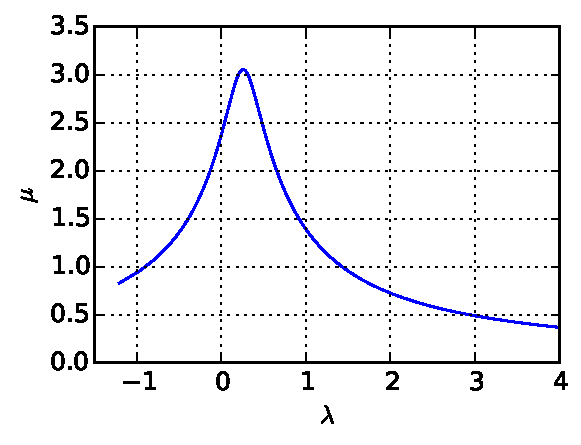
\includegraphics{theorie/graphe/alpha_4.pdf}
		\caption{Courbe calorique du modèle isotherme idéalisé possédant un halo de pente $-4$ \label{fig::DET}}
	\end{figure}

	Cette courbe présente bel et bien une tangente horizontale, en $x^*_4= \frac{1}{4} \left(5+\sqrt{5}\right) \approx 1.81$, qui correspond à une
	instabilité dans l'ensemble canonique dans le cadre de notre calcul (bain thermique). Le contraste de densité correspondant est
	$\mathcal{R}_4\approx 10.71$

\subsection{Conclusion du modèle}

	Une conclusion raisonnable de cette étude est qu'un système cœur-halo dont le contraste de densité est plus important que $\mathcal{R}_4$ est
	instable s'il est entouré d'un bain thermique de même température que la sphère. Cette instabilité conduit à l'effondrement du cœur du
	système.

	Cette instabilité pourrait être à l'origine de l'absence de cœur dans le résultat de l'effondrement d'un système inhomogène.

	La courbe calorique peut être calculée dans les mêmes conditions pour des systèmes cœur-halo de pentes différentes. Nous les avons rassemblé
	sur la figure~\ref{ToyModel::AllAlpha}.
	\begin{figure}
			\centering 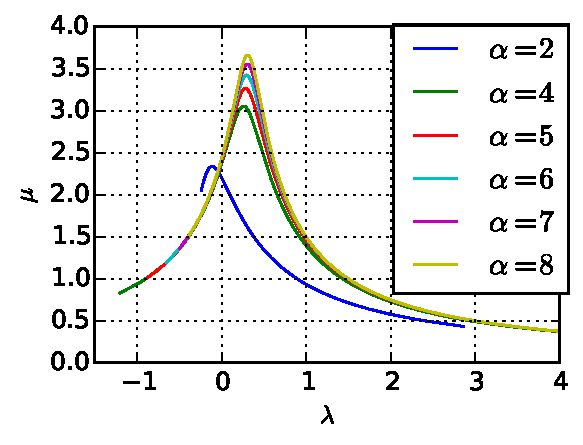
\includegraphics{theorie/graphe/alpha_all.pdf}
			\caption{Courbe calorique pour des systèmes cœur--halo de pente $\alpha=4, 5, 6, 7, 8$\label{ToyModel::AllAlpha}}
	\end{figure}
	La même instabilité est toujours présente. Dans le cas $\alpha=2$, les calculs sont identiques, il conduisent au couple:
	\begin{eqnarray}
		\mu(x) =& \frac{10 (3x-2) (x-1)}{x(15x-14-10\ln(x))} \\
		\lambda(x) =& -\frac{3x(15x-14-10\ln(x))(x-2)}{20(x-1)(3x-2)^2}
	\end{eqnarray}
	Nous remarquons que $\lim(\lambda,\mu)_{x\to\infty}=(-\frac{1}{4},2)$ correspond bien à la spahère isotherme. La tangente verticale n'a pas
	résisté à l'idéalisation, par contre la tangente horizontale reste présente pour une valeur $x^*_2=3.48$ correspondant à un contraste de
	densité $\mathcal{R}_2= 12.1$. Cette valeur est environ trois fois plus petite que la valeur exacte (32.1) mais la transition stable/instable
	est bien respectée par le modèle approché. Il semble légitime de penser que la valeur de $\mathcal{R}_4$ trouvée pour le modèle cœur-halo de
	pente -4 soit également un peu sous-estimée.
